\documentclass[a4paper,11pt]{article}
%Premeable
	%Chinese
	\usepackage[UTF8,fontset=fandol]{ctex}
	\usepackage{xeCJK}
	\usepackage[datesep=/]{datetime2}
	\DeclareTextFontCommand{\textbf}{\sffamily}
%Presenting
	\usepackage[table]{xcolor}
	\usepackage{graphicx}
	\usepackage[font={sf}]{caption}
	\usepackage[above]{placeins}
	\usepackage{float,wrapfig}
	\usepackage{tabularx,array,booktabs,multirow,bigstrut}
	\newcolumntype{C}[1]{>{\hsize=#1\hsize%
		\centering\arraybackslash}X}
	\newcommand{\minitab}[2][l]{%
		\begin{tabular}{#1}#2\end{tabular}}
%MathSetting
	\let\latexointop\ointop
	\usepackage{amsmath,bm,amssymb,esint,extarrows}
	\usepackage{upgreek,textcomp,mathrsfs}
	\usepackage[only,sslash]{stmaryrd}
	\usepackage{nicefrac,eqnarray}
%	\usepackage{amsthm}
	\usepackage{mathtools,physics,siunitx}
	\usepackage{stackengine,titling,varwidth}
	\usepackage{tikz}
	\usepackage{resizegather,empheq}
	\usetagform{default}
	\usepackage{calligra,fourier-orns}
	% Keep \oint unchanged by esint
	\let\ointop\undefined
	\let\ointop\latexointop
	% Define a scriptr 
	\DeclareMathAlphabet{\mathcalligra}{T1}{calligra}{m}{n}
	\DeclareFontShape{T1}{calligra}{m}{n}{<->s*[2.2]callig15}{}
	\newcommand{\scriptr}{\mathcalligra{r}\,}
	\newcommand{\rvector}{\pmb{\mathcalligra{r}}\,}
	% Useful shorthand
	\DeclarePairedDelimiter\ave{\langle}{\rangle}
	\newcommand\inlineeqno{\stepcounter{equation}\ (\theequation)}
	\newcommand{\sinc}{\operatorname{sinc}}
	\newcommand{\mbb}[1]{\mathbb{#1}}
	\newcommand{\mrm}[1]{\mathrm{#1}}
	\newcommand{\mcal}[1]{\mathcal{#1}}
	% Scaling and positioning
	\newcommand\scalemath[2]{\scalebox{#1}{\mbox{\ensuremath{\displaystyle #2}}}}
	\newcommand\raisemath[2]{\raisebox{#1\depth}{${#2}$}}
	\empheqset{box=\bbox}
	% Presenting
	\newcommand*\bbox[1]{\fbox{\hspace{1em}\addstackgap[5pt]{#1}\hspace{1em}}}
	\sisetup{%
		redefine-symbols=false,%
		separate-uncertainty=true,%
		range-phrase=\,\textasciitilde\,,%
		arc-separator = \,}
	\allowdisplaybreaks[2]
%ParagraphSetting
	\setlength{\parskip}{.3\baselineskip}
	\usepackage[defaultlines=2,all]{nowidow}
	\postdisplaypenalty=50
%PageSetting
	\usepackage[colorlinks=true,linkcolor=blue]{hyperref}
	\usepackage[vmargin={4cm,5cm},hmargin=3cm,%
		footnotesep=\baselineskip]{geometry}
	\usepackage[bottom]{footmisc}
	\usepackage{changepage}
	% Autoref names
	\renewcommand{\tableautorefname}{\tablename}
	\renewcommand{\figureautorefname}{\figurename}
	% List settings
	\usepackage{enumitem}
	\setlist{itemsep=0pt,topsep=0pt,labelindent=\parindent,leftmargin=0pt,itemindent=*}
	% Some redefined lengths
	\setlength{\headsep}{2.2cm}
	\setlength{\droptitle}{-2.2cm}
	\setlength{\footnotesep}{3\parskip}
	% Header
	\usepackage{fancyhdr,lastpage}
	\pagestyle{fancy}
	\fancyhf{}
	\cfoot{--\ \thepage\,/\,\pageref{LastPage} \ --}
	\renewcommand{\headrulewidth}{0.1pt}
	\renewcommand{\headrule}{
		\vbox to 2pt{
		\hbox to \headwidth{\dotfill}\vss}}
	% Separator
	\newcommand{\newparagraph}{\pagebreak[3]\noindent%
		\hfil
		~\raisebox{-4pt}[10pt][10pt]{\decofourright~~~~~~~~\decofourleft}~ %
		\par
	}
%TitleSettings
	\pretitle{\begin{center}}
	\posttitle{\par\end{center}\vspace{-6mm}}
	\predate{}
	\postdate{\vspace{-4mm}}
%Header
	\lhead{%
		
\includegraphics[height=3.2em]{PKUPhy.png}
		\vspace{-3ex}
		}
	\rhead{%
		\itshape\small
		\begin{tabular}{rr}
			\multicolumn{2}{r}{赵启渊} \\[.3em]
			学号:   & 2000011153 \\[.2em]
		\end{tabular}\hspace{-1em}
		}
%Title
	\title{\textit{\large 实验十七}\\[2mm]
		\textbf{\LARGE RLC电路的谐振现象}}
	\author{\textit{赵启渊} 2000011153}
	\date{}
%Miscellaneous
	\newcommand{\tabindent}{\hspace{2em}}
%FourierTransform
	\newcommand{\ftransform}{\xlongrightarrow{\ \mathscr F\ }}
	\newcommand{\iftransform}{\xlongrightarrow{\ \mathscr F^{-1}\ }}
	\usepackage{gensymb}

\begin{document}
	\vspace*{1cm}
	
	\vspace*{1cm}
	
	\begin{center}
		\Huge{\textbf{基础物理实验报告}}
		
		\Large{RLC电路的谐振现象}
	\end{center}
	
	\vspace*{2cm}
	
	\begin{table}[h]
		\centering	
		\begin{Large}
			\begin{tabular}{p{3cm} p{7cm}<{\centering}}
				姓\qquad 名: & 赵启渊 \\
				\hline
				学\qquad 院: & 工学院 \\
				\hline
				学\qquad 号: & 2000011153 \\
				\hline
				分\qquad 组: & 第1组7号 \\
				\hline
				日\qquad 期: & 2022年3月30日 \\
				\hline
				指导教师: & 刘春玲\ 张艳席\\
				\hline
			\end{tabular}
		\end{Large}
	\end{table}
	
\maketitle
\thispagestyle{fancy}
\section{数据及处理}
\subsection{测量谐振下的电压值}
	按下面电路图连接电路,取L=0.1H、C=0.05$ \mu F  $、R=100$ \ohm $,示波器CH1连接C上方导线,示波器CH2连接R上方导线,注意CH1和CH
	2必须共地,调谐振,用数字万用表测量$u,u_{L},u_{C},u_{R}$。
	\begin{figure}[H]
		\centering
		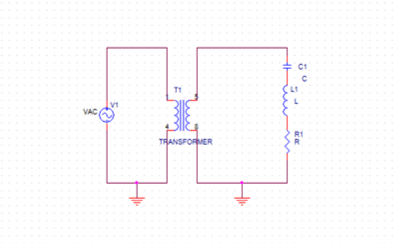
\includegraphics[width=.6\linewidth]{图片1.png}
		\caption{RLC串联电路图}
	\end{figure}\noindent%

	测量得$$ f_{0} = 2.249 kHz $$
	
	\begin{table}[H]
		\centering\caption{测量谐振条件下的电压值}
		\small
		\begin{tabularx}{.85\linewidth}{C{1} *6{C{.8}}}
			\toprule
			\textbf{项目} &
			$u / \si{\V}$ &
			$u_{L}/ \si{\V}$ &
			$u_{C} / \si{\V}$ &
			$u_{R} / \si{\V}$ & \\
			\midrule
			读数     & 0.6705  & 7.194  & 7.172 & 0.5151 &   \\
			\bottomrule
		\end{tabularx}
		\vspace{3ex}
	\end{table}\noindent%

    因为在共振时,电阻、电容两端电压会相互抵消,相当于整个电压都加到了R上,由此可以算出整个电路总电阻$$ R^{\prime} = \frac{u}{u_{R}} * R $$
	$$ R^{\prime} = 131.04 \ohm $$
	由此得品质因子
	$$ Q_{1} = \dfrac{1}{R^{\prime} * C * \omega_{0}} $$
	$$  = \dfrac{1}{ 2* \pi * R^{\prime} * C * f_{0}} $$
	$$  = 10.8 $$
	$$ Q_{2} = \dfrac{u_{C}}{u} $$
	$$ Q_{2} = 10.70 $$

\subsection{绘制电路的相频特征曲线}
通过调节信号源,发生一定频率梯度的脉冲电压,用示波器测量CH1、CH2过零点之间的时间差$\Delta t$,计算得到相位差$\Delta \phi$,最后绘图。
	\begin{table}[H]
	\centering\caption{测量不同频率下时间差的数据表}
	\small
	\begin{tabularx}{.85\linewidth}{C{1} *6{C{.8}}}
	\toprule
		输出频率 / \si{\kHz} &
		$\Delta t  / \si{\ms}$ &
		$\Delta \phi / \si{\degree}$ &\\
	\midrule
	     1.741  & 0.128  & -80.2    \\
		 1.955  & 0.100  & -70.4    \\
		 2.078  & $80.0 * 10^{-3}$  & -59.8  \\
		 2.148  & $56.0 * 10^{-3}$  & -43.3  \\
	   	 2.190  & $37.0 * 10^{-3}$  & -29.2  \\
		 2.221  & $17.0 * 10^{-3}$  & -13.6  \\
		 2.249  & $1.00 * 10^{-3}$  & 0.80  \\
		 2.276  & $23.0 * 10^{-3}$  & 18.8  \\
		 2.309  & $39.0 * 10^{-3}$  & 32.4  \\
		 2.354  & $57.0 * 10^{-3}$  & 48.3  \\
		 2.434  & $71.0 * 10^{-3}$  & 62.2  \\
		 2.587  & $78.0 * 10^{-3}$  & 72.6  \\
		 2.905  & $75.0 * 10^{-3}$  & 78.4  \\
		
	\bottomrule
	\end{tabularx}
	\vspace{3ex}
	\end{table}\noindent%
    其中$\Delta \phi$计算使用$$ \Delta \phi = \Delta t * f * 360 \degree $$
	以频率f为横坐标,相位差$\Delta \phi$为纵坐标绘图得
	\begin{figure}[H]
		\centering
		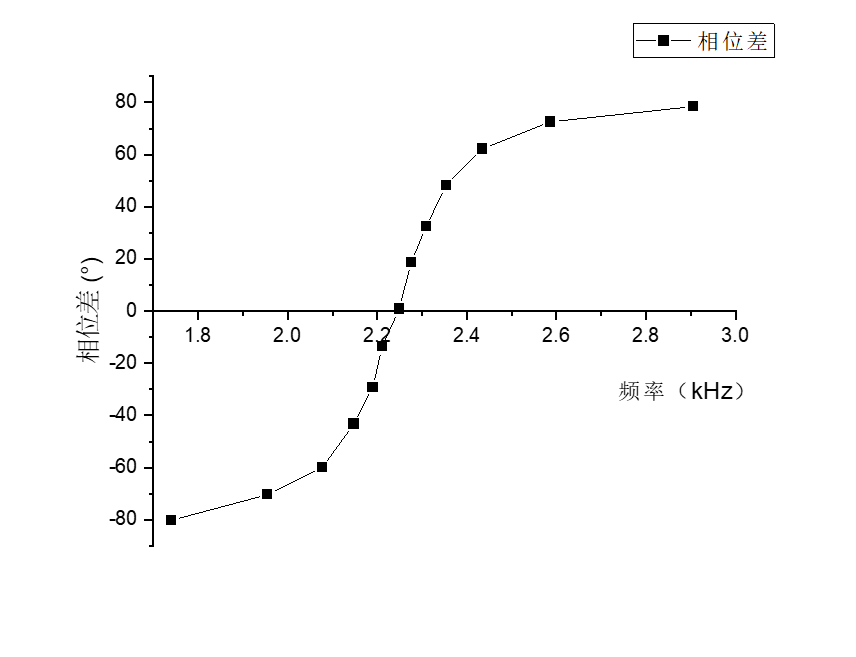
\includegraphics[width=.6\linewidth]{图片2.png}
		\caption{RLC串联电路相频特征曲线}
	\end{figure}\noindent%
	
\subsection{绘制电路的幅频特征曲线}
通过调节信号源,在总电压$u = 1.0000 \pm 0.001 V$的条件下,发生上面的频率梯度的脉冲电压,并在每个频率梯度之间再取一点,共取25个点,每点用数字万用表测量$ u_{R}$,计算得到$i$值,最后绘图,并用带宽法计算品质因子$Q$的值 。
\begin{table}[H]
	\centering\caption{测量不同频率下$ u_{R}$值的数据表}
	\small
	\begin{tabularx}{.85\linewidth}{C{1} *6{C{.8}}}
		\toprule
		输出频率 / \si{\kHz} &
		$u_{R}  / \si{\mV}$ &
		输出频率 / \si{\kHz} &
		$u_{R}  / \si{\mV}$ &\\
		\midrule
		1.741  & 134.73  & 2.262  & $0.7616 * 10^{3}$ \\
		1.848  & 174.64  & 2.276  & $0.7465 * 10^{3}$ \\
		1.955  & 239.70  & 2.292  & $0.6975 * 10^{3}$ \\
		2.016  & 306.36  & 2.309  & $0.6627 * 10^{3}$ \\
		2.078  & $0.3878 * 10^{3}$  & 2.331  & $0.5818 * 10^{3}$  \\
		2.113  & $0.4480 * 10^{3}$  & 2.354  & $0.5431 * 10^{3}$  \\
		2.148  & $0.5468 * 10^{3}$  & 2.394  & $0.4483 * 10^{3}$ \\
		2.170  & $0.6110 * 10^{3}$  & 2.434  & $0.3845 * 10^{3}$ \\
		2.190  & $0.6682 * 10^{3}$  & 2.510  & 281.08 \\
		2.205  & $0.7102 * 10^{3}$  & 2.587  & 238.24 \\
		2.221  & $0.7395 * 10^{3}$  & 2.746  & 165.53 \\
		2.235  & $0.7632 * 10^{3}$  & 2.905  & 134.19 \\
		2.249  & $0.7752 * 10^{3}$  & \\
		\bottomrule
	\end{tabularx}
	\vspace{3ex}
\end{table}\noindent%
其中$i$计算使用$$ i = \dfrac{u_{R}}{R} $$
以频率f为横坐标,电流值$i$为纵坐标绘图得
\begin{figure}[H]
	\centering
	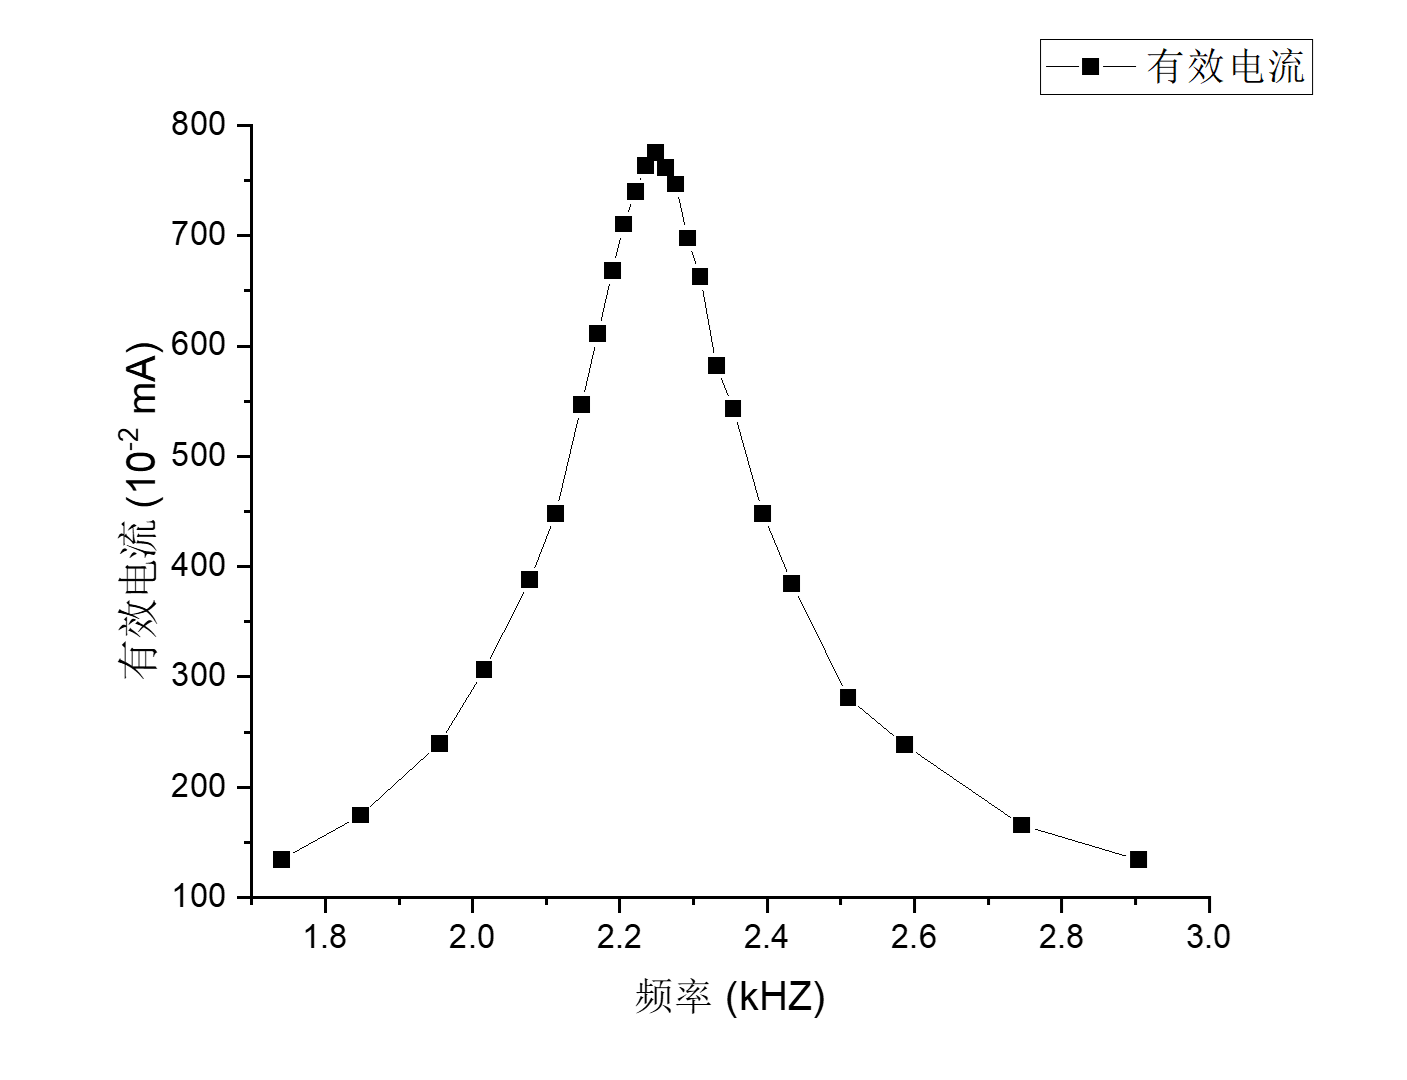
\includegraphics[width=.6\linewidth]{图片3.png}
	\caption{RLC串联电路幅频特征曲线}
\end{figure}\noindent%
又因为$$ \frac{i_{max}}{\sqrt{2}} = 548.1 * 10^{-2} mV$$
使用Origin在曲线上取$A(2.14825,548.0) , B(2.35034,548.0)$两点,计算得$$ Q_{3} = \dfrac{f_{0}}{\Delta f} $$
	$$  = \dfrac{f_{0}}{2.35034 - 2.14825} $$
	$$  = 11.00 $$
\section{思考题:}
\ \\
2.\\

(1)当谐振时,电路中会有关系
\begin{equation}
	 Q = \dfrac{u_{C}}{u} 
\end{equation}
\begin{equation}
	\left\{
	\begin{array}{c}
		L = \dfrac{1}{\omega_{0}^{2} * C} \\
		\omega_{0} = 2 * \pi * f_{0} \\
	\end{array}
	\right.
\end{equation}
\begin{equation}
	\left\{
	\begin{array}{c}
		R_{r} = \dfrac{1}{Q * \omega_{0} * C} \\
		\omega_{0} = 2 * \pi * f_{0} \\
	\end{array}
	\right.
\end{equation}
其中$ C $、$ f_{0} $、 $ u_{C} $、 $ u $都是可以从Q表中测量得到的,通过上面的方程就可以得到想要的参数。

(2)\begin{enumerate}
	\item 按照Q表原理图连接电路,调节输出频率,使整个电路处于谐振状态。
	\item 读出谐振频率$f_{0}$、$u_{C}$、$u$,再根据仪器给出的参数$C$,就可以得到电抗元件的$R_{r}$、$L$ 、$Q$的值。 
	
\end{enumerate}

(3)因为
$$
	Q = \dfrac{u_{C}}{u} 
$$
得到
$$ Q = 1.0 * 10^{2}$$
因为
$$
	\left\{
	\begin{array}{c}
		L = \dfrac{1}{\omega_{0}^{2} * C} \\
		\omega_{0} = 2 * \pi * f_{0} \\
	\end{array}
	\right.
$$
得到
$$ L = 0.21 mH$$
因为
$$
	\left\{
	\begin{array}{c}
		R_{r} = \dfrac{1}{Q * \omega_{0} * C} \\
		\omega_{0} = 2 * \pi * f_{0} \\
	\end{array}
	\right.
$$
得到
$$ R_{r} = 8.0 \ohm $$






\section{分析与讨论}
\subsection{实验测得各种曲线的主要特征与理解}
\begin{enumerate}
	\item 对于RLC串联电路的相频特征曲线,有方程
	\begin{equation}
		\phi = arctan{\dfrac{2*\pi*f * L - \frac{1}{2*\pi*f * C}}{R}} 
	\end{equation}
	当电流与电压相位相同时,这时的频率就是谐振频率;当$ f < f_{0} $时,这时候频率较低,电流的相位超前于电压的相位,整个电路呈现电容性,并且随着$ f $的减小,相位差趋近于$ \frac{\pi}{2} $;当$ f > f_{0} $时,这时候频率较高,电流的相位落后于电压的相位,整个电路呈现电感性,并且随着$ f $的增大,相位差趋近于$ \frac{\pi}{2} $。
	
	\item 对于RLC串联电路的幅频特征曲线,有方程
	\begin{equation}
		i= \dfrac{u}{\sqrt{R^{2} + (2*\pi*f * L - \frac{1}{2*\pi*f * C}) ^{2}}} 
	\end{equation}
    从方程和测得的曲线得到,该曲线是对称的,在谐振时,总阻抗$ \left | Z \right |$最小,因此此时有$ i_{max} $。随着$ \left | f-f_{0} \right |$越来越大,总阻抗$ \left | Z \right |$值增大,i减小,并且i衰减的速度先加快后减慢。并且直观上,从图像的形状上可以反应Q值的大小,高而瘦的Q值大,矮而胖的Q值小。
    
	
	
\end{enumerate}
	
\subsection{比较三种方法测得的Q值}
$$ Q_{1} = 10.8 $$
$$ Q_{2} = 10.70 $$
$$ Q_{3} = 11.0 $$
三种方法测得的Q值是大致一样的。下面对三种方法测得的Q值进行不确定度分析。
\begin{enumerate}
	\item $$ Q_{1} = \dfrac{1}{ 2* \pi * R^{\prime} * C * f_{0}} $$
	$$ \frac{dQ}{Q} = - \frac{du}{u} + \frac{du_{R}}{u_{R}} - \frac{dR}{R} - \frac{df_{0}}{f_{0}} - \frac{dC}{C}$$
	$$ \frac{\sigma Q}{Q} =\sqrt{  (\frac{\sigma u}{u})^{2} + (\frac{\sigma u_{R}}{u_{R}})^{2} + (\frac{ \sigma R}{R})^{2} + (\frac{\sigma f_{0}}{f_{0}})^{2} + (\frac{\sigma C}{C}})^{2} $$
	$$ \sigma Q_{1} = 5.16 * 10^{-3} $$
	\item $$ Q_{2} = \dfrac{ u_{C} }{ u } $$
	$$ \frac{dQ}{Q} = - \frac{du}{u} + \frac{du_{C}}{u_{C}} $$
	$$ \frac{\sigma Q}{Q} =\sqrt{  (\frac{\sigma u}{u})^{2} + (\frac{\sigma u_{C}}{u_{C}})^{2}} $$
	$$ \sigma Q_{2} = 2.36 * 10^{-3} $$
	\item $$ Q_{3} = \dfrac{f_{0}}{\Delta f} $$
	$$\frac{dQ}{Q} =  \frac{df_{0}}{f_{0}} - \frac{d\Delta f}{\Delta f}$$
	$$ \frac{\sigma Q}{Q} =\sqrt{  (\frac{\sigma f_{0}}{f_{0}})^{2} + (\frac{\sigma \Delta f}{\Delta f})^{2}} $$
	$(\frac{\sigma \Delta f}{\Delta f})^{2}$来自图形拟合的误差和测量电压的误差,其中图形拟合的误差是非常大的,可能造成$ \sigma Q $很大。
	\item 由于图形拟合的误差,$ \sigma Q_{3} $是三种测量方法中最大的;其次由于第一种方法测量的变量很多,$ \sigma Q_{1} $是居中的;$ \sigma Q_{2} $是最小的,第二种方法应该是最精确的。但总体来说,三种方法测量的Q值都比较集中,说明测量比较精准。
\end{enumerate}
	
\section{收获与感想}
\begin{enumerate}
	\item 在做电学实验时,一定要预先检查电路,避免短路。在本实验中要注意避免地的选择不共点,导致短路。
	\item 选择测量方案时,要尽量选择测量数量少的,避免因为实验仪器的误差造成很大的误差。
	\item RLC电路在实际应用中,Q越大,对电路电压的放大作用越大,这可以在现实中用作放大器。
\end{enumerate}

\begin{appendix}
	\section{对未知电路盒的元件参数测定}
	\subsection{实验原理:}
	\begin{enumerate}
	\item 该未知电路盒是电阻、电容、电感三种元件中两种的组合,电容、电感需要考虑损耗电阻。在同时具有电容、电感的电路中有一定几率出现谐振现象。电容在电路中会通高频,阻低频;电感在电路中会通低频,阻高频。按下面的电路图搭建电路,这里$R = 100 \ohm$。
	\begin{figure}[H]
		\centering
		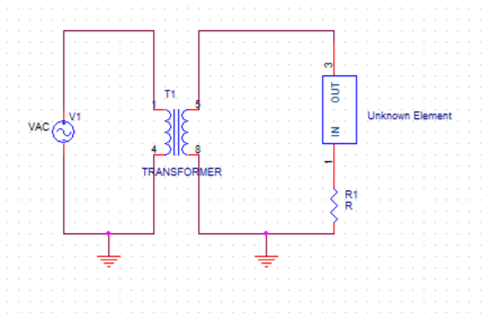
\includegraphics[width=.6\linewidth]{图片4.png}
		\caption{未知电路盒的元件参数测定的电路图}
	\end{figure}\noindent%
    示波器CH1连接未知电路盒的上方导线,示波器CH2连接R上方导线,注意CH1和CH2必须共地,用数字万用表测量$u_{R}$。首先调谐振,若存在谐振现象,则一定存在电容与电感;若不存在谐振现象,则有两种可能:电容与电阻、电感与电阻。之后根据电容、电感的特性,用高频电流与低频电流分别检验$u_{R}$,再判断未知电路盒的类型。
    \item 对于元件参数的测量,要使用谐振电路的特性,对于不存在谐振现象的有两种可能,要构造谐振电路,用带宽法测量未知电路盒的参数。$$
    Q = \dfrac{f_{0}}{\Delta f} $$
    $$ R^{\prime} = \frac{u}{u_{R}} * R $$
    $$ Q = \dfrac{1}{R^{\prime} * 2* \pi *f_{0}* C} $$
    $$ Q = \dfrac{ 2* \pi *f_{0}* L}{ R^{\prime} } $$
    \end{enumerate}
    \subsection{实验步骤:} 
    \begin{enumerate}
    	\item  按实验原理中的电路图连接电路(使用(7)号器件盒),不断调节输出频率,发现在$ f_{0} = 3.100 kHz $时,示波器中的李萨如图形基本为一直线,电路发生谐振现象。说明该器件盒存在电容和电感。
    	\item 笔者又采用定性实验的方法,测量在输出电压为1.768 V,输出频率为200Hz时,$u_{R}$的量级为50mV;测量在输出电压为1.768 V,输出频率为1MHz时,$u_{R}$的量级为10mV。可以发现$u_{R}$在高低频时负载的电压极小,可以进一步说明该器件盒存在电容和电感。
    	\item 再次调谐振,测量$u$、$u_{R}$的值,从而计算$R^{\prime}$。
    	\item 再次调谐振,保持实验电路的总电压为$u = 1.0000 \pm 0.001 V$,测量$u_{R}$。不断调节输出频率,并保持实验电路的总电压为$u = 1.0000 \pm 0.001 V$,测量此时的$u_{R}$,使其不断接近$\dfrac{u_{max}}{\sqrt{2}}$ 。
    	\item 计算数据,得到位置元件的参数。
    \end{enumerate}  
    \subsection{实验数据处理:} 
    \begin{enumerate}
    	\item  测量得到$$ f_{0} = 3.100 kHz $$
    	\item 测量得到$$u_{R} = 0.9051 V$$
    	$$u = 1.1330 V$$
    	计算得$$R^{\prime} = \dfrac{u}{u_{R}} * R$$
    	$$ = 125.18 \ohm$$
    	损耗电阻
    	$$ \Delta R = R^{\prime} - R$$
    	$$ = 25.18 \ohm$$
    	\item 测量得到
    	\begin{table}[H]
    		\centering\caption{测量不同频率下$ u_{R}$值的数据表}
    		\small
    		\begin{tabularx}{.85\linewidth}{C{1} *6{C{.8}}}
    			\toprule
    			输出频率 / \si{\kHz} &
    			$u_{R}  / \si{\mV}$ &\\
    			\midrule
    			3.100  & $0.7990 * 10^{3}$   \\
    			2.120  & $0.5125 * 10^{3}$   \\
    			2.148  & $0.5286 * 10^{3}$   \\
    			2.170  & $0.5324 * 10^{3}$   \\
    			2.175  & $0.5343 * 10^{3}$    \\
    			2.235  & $0.5596 * 10^{3}$    \\
    			2.240  & $0.5612 * 10^{3}$    \\
    			\bottomrule
    		\end{tabularx}
    		\vspace{3ex}
    	\end{table}\noindent%
    	\item $$\dfrac{u_{max}}{\sqrt{2}} = 0.5650 V$$ 
    	观察到输出频率为2.240kHz时,$u_{R}$较为接近,粗略计算有
    	$$ Q = \dfrac{f_{0}}{\Delta f} $$
    	$$  = \dfrac{f_{0}}{2 * (f_{0} - f)} $$
    	$$  = 1.802 $$
    	因此有
    	$$ C = \dfrac{1}{2 * \pi * f_{0} * R^{\prime} * Q} $$
    	$$  = 0.2276 \mu F  $$
    	$$ L = \dfrac{Q * R^{\prime}}{2 * \pi * f_{0} } $$
    	$$  = 0.01158 H  $$
    \end{enumerate}    
\end{appendix}

	\vfill\noindent\itshape\footnotesize
	\hfill Last edited: \today\ \copyright\ 赵启渊
\end{document}